\title{LEZIONE 1 11/03/20}\newline
\textbf{link} \href{https://web.microsoftstream.com/video/58568b1d-5fc5-41c0-88f6-608e4b8f9f7a}{clicca qui}
\section{Architetture}
Il web è una piattaforma per sviluppo di applicazioni con un architettura molto particolare. Per \textbf{architettura} si intende l'insieme delle risorse (hardware, connettività, software di base, software applicativo).\newline
\newline 
Le architetture sono  cambiate molto negli anni. Se ne individuano tre grandi famiglie: Mainframe, Client-Server, Multi-tier.\newline
Le applicazioni web sfruttano l'architettura Three-tiers che prevede tre livelli: Client, Middle-tier, Data-tier.\newline
Lo scopo di questa prima metà di corso è quello di riuscire a programmare nel \textbf{Middle-tier}. Il Middle-tier si occupa di centralizzare la connesione ai database servers, maschera il modello dei dati al cliente e in genere può avere funzionalità varie di complessità anche elevata.\newline
\newline
In un'applicazione web il Client interagisce con il Middle-tier con un preciso protocollo, che non è il classico TCP-IP, ma, nel nostro caso, è il protocollo HTTP.\newline
\newline
Una lettura molto importante per il corso è il documento RequestforComment 1945, Tim Berners Lee (\url{https://www.w3.org/Protocols/rfc1945/rfc1945}), che rappresenta l'atto di fondazione del web.]\newline
\newline
Il meccanismo principale del protocollo HTTP consiste in requests mandate dal Client al Server, che a sua volta invia delle responses. Le request del Client sono gestite tramite un applicazione detta User agent (browser).\newline
Http è rivoluzionario per la sua \textbf{semplicità}: le richieste del Client e le risposte del Server sono delle semplici stringhe. \newline
\newline
Architettura delle applicazioni web: c'è un \textbf{Client} (pc) con un \textbf{user agent} (browser) che emette \textbf{richieste} (HTTP request) che vengono servite con delle \textbf{risposte} (HTTP response) dal Middle-tier, in particolare da un \textbf{web server}, detto anche \textbf{HTTP server}.\newline
L'archiettura di cui ci occupiamo è, però, più complicata di così, il Middle-tier prevede alle spalle del web server un \textbf{application server} (TomCat), che ha lo diverse funzionalità, fra le quali, per esempio, quella di calcolare una risposta "personalizzata" secondo parametri e criteri precisi e di produrre un pagina web appropriata o di connettersi ai database SQL e di interagirci.\newline
L'application server a sua volta risiede in un \textbf{origin server}, che è il server nel quale le risorse risiedono (o vengono create).\newline
\newline
Altri elementi dell'architettura sono poi il proxy e il gateway.\newline
Il \textbf{proxy} è un intermediario fra un client e un origin server, per definizione può comportarsi sia come server sia come client. Fa copie di risorse e le inoltra ai client e può essere anche utile per limitare gli accessi e gestire autorizzazioni.\newline
Il \textbf{Gateway} è colui che agisce da intermediario per altri server ed è tipicamente utilizzato per far interagire un applicazione web con applicazioni che non usano il protocollo HTTP: il gateway traduce richieste HTTP per applicazioni che non lo comprendono, come i sistemi SQL.
\begin{center}
    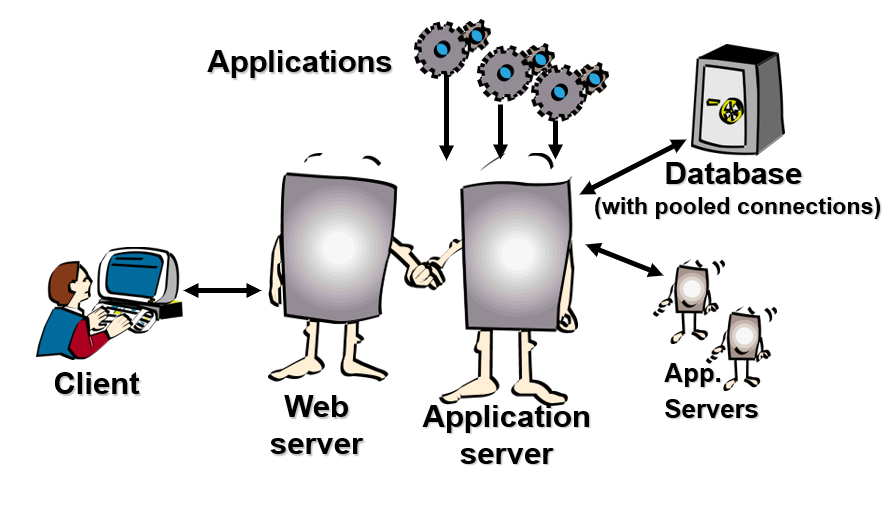
\includegraphics[height=4cm]{../lezione1/img1.PNG}
\end{center}
\newpage
\section{HTTP}
HTTP sta per \textbf{HyperText Transfer Protocol}.\newline
\newline
HTTP è \textbf{stateless}, cioè ogni ciclo di richiesta-risposta è indipendente, non si preserva alcun tipo di dato fra connessioni diverse. Essendo stateless è anche \textbf{sessionless}.\newline
Al contrario l'application server può essere \textbf{statefull} e di conseguenza essere \textbf{sessionfull}.\newline
\newline
Come si identifica una risorsa? con l'\textbf{URL} (Uniform Resourse Locator) che è una striga formatta (\textbf{structured string}) in maniera molto semplice:
\begin{itemize}
    \item prefisso (protocollo): \textbf{"http"};
    \item \textbf{"//"};
    \item indicazione della macchina fisica in cui è presente la risorsa con una eventuale porta in cui la macchina ascolta le richieste: \textbf{host[":"port]};
    \item un path (opzionale): \textbf{[abs\_path]};
\end{itemize}
\subsection{HTTP request} 
L'HTTP request una banale stringa che contiene una \textbf{request-line}, degli \textbf{header} e un allegato opzionale, detto \textbf{body}.\newline
La request-line contiene tre informazioni: il \textbf{metodo} (funzione) della richiesta, l'\textbf{URL}, la \textbf{versione del protocollo} usata. I metodi di richiesta sono principalmente due, GET e POST; questi metodo possono essere visti come chiamate di funzione.
\subsection{HTTP response} 
Anche l'HTTP response è una banale stringa, che, ancora più semplicemente contiene solo: un \textbf{codice di stato} (es. 404 file not found), degli \textbf{header} facoltativi, e un allegato, anche qui chiamato \textbf{body}.\newline
I codici di stato si classificano in base alla loro prima cifra: 1 informativi, 2 successo, 3 reindirizzamento, 4 errore nel client, 5 errore nel server.\newline
\newline
Gli header sono informazioni opzionali a cura del browser, trasmesse come fossero parametri che aggiungono informazioni alla request o alla response.\newline
\newline
La conseguenza di un protocollo così semplice è che con un solo identico client si può interagire con tanti back end differenti. La complessità si sposta però nell'application server, a carico del programmatore.
\newpage
\section{CGI}
CGI sta per \textbf{Common Gateway Interface} ed è una tecnologia ormai deprecata e superata.\newline
\newline
CGI nasce a fronte del problema di creare applicazioni web dinamiche e personalizzate in base alle richieste inviate dal client. Il problema che si pone di risolvere era l'impossibilità di comunicare i parametri HTTP presenti nella request al programma (che "gira" su un altro thread) che si occupa della creazione della response (del file HTML personalizzato).\newline
\newline 
CGI è, quindi, un'interfaccia che permette al web server di eseguire applicazioni esterne che creino pagine dinamiche. Questa interfaccia è implementata tramite un certo numero di \textbf{variabili d'ambiente} (condivisibili fra più processi) standardizzate, nelle quali il web server può salvare le informazioni di un richiesta HTTP in modo che siano in una zona di memoria alla quale un processo di un applicazione esterna può accedere.\newline
\newline
Vediamo il tipico work-flow di un applicazione che sfrutta CGI: innanzitutto l'URL della richiesta HTTP presenta un path che porta a un applicazione \textbf{eseguibile} (.exe), il web server intercetta la richiesta e smonta (fa il parsing) la richeista, ne preleva le informazioni (i parametri) e le salva nelle variabili d'ambiente, successivamente invoca l'eseguibile. L'application server può ora prelevare le informazioni necessarie dalle variabili d'ambiente e costruire un file HTML appropriato, che verrà mandato come risposta al client.\newline
\newline
CGI ha due grandi \textbf{difetti}, il primo riguarda la \textbf{sicurezza}, in quanto i file eseguibili erano direttamente accessibili, il secondo è che siccome i \textbf{processi} dell'application server \textbf{muoiono} dopo ogni esecuzione, non c'è modo di creare un sistema che mantenga una \textbf{sessione} attiva. Inoltre le prestazioni di CGI sono molto scarse, per esempio, siccome i processi muoiono continuamente, c'è un continuo bisogno di stabilire connessioni coi database, che è un operazione onerosa.\newline